\documentclass[12pt]{csethesis}
\usepackage[english]{babel}
\usepackage{amsmath}        % Extra math definitions
\usepackage{graphics}       % PostScript figures
\usepackage{setspace}       % 1.5 spacing
\usepackage{multicol}
\usepackage{bigints}
\usepackage{amssymb}
\usepackage{graphicx}
\usepackage{subcaption}
\usepackage{footnote}
\usepackage{lscape}
\usepackage{color}
\usepackage{array}
\usepackage{multirow}
\usepackage{sidecap}
\usepackage[table]{xcolor}
\usepackage{colortbl}
\usepackage{sidecap}
\usepackage{longtable}
\usepackage{wrapfig}
%\usepackage{hyperref}
\newtheorem{lemma}{Lemma}[chapter]
\makeatletter
\@addtoreset{lemma}{chapter}
\makeatother
\newtheorem{theorem}{Theorem}[chapter]
\makeatletter
\@addtoreset{theorem}{chapter}
\makeatother

\usepackage[left=1.5in,right=1in,top=1in,bottom=1in]{geometry}
%\usepackage[top=1cm,left=1cm,right=1cm,bottom=1cm]{geometry}
\usepackage{emptypage}
\usepackage{lipsum}
\usepackage{fancyhdr}
%\fancyfoot{}
%\fancyfoot{\thepage}
\fancyhead[RO,LE]{}
\fancyhead[RE]{\ifnum\value{chapter}>0 \bfseries{\nouppercase{\rightorleftmark}} \else \bfseries{\leftmark} \fi}
\fancyhead[LO]{\ifnum\value{chapter}>0 \bfseries{\nouppercase{\rightorleftmark}}  \else \bfseries{\leftmark} \fi}
%\fancyhead[LO]{ \bfseries\slshape\nouppercase{\rightorleftmark}}
\makeatletter
\newcommand{\rightorleftmark}{%
  \begingroup\protected@edef\x{\rightmark}%
  \ifx\x\@empty
    \endgroup\slshape\nouppercase{\leftmark}
  \else
    \endgroup\rightmark
  \fi}
\makeatother

\newtheorem{example}{Example}
\phdtitle = {[Title of the project]}
\name = {[Name of the student]}
\rollno = {[Roll Number]}
\guide = {[Name of Supervisor]}

\begin{document}
\pagenumbering{roman}
\begin{titlepage}
% \textheight 15.5in \textwidth 12.5in {\raggedright \huge\bf \the\phdtitle}\\[70ex]
% \begin{flushright}
% \hspace{8cm}{\LARGE \bf \the\name}\\  [1ex] 
% \end{flushright}
%\pagebreak
\thispagestyle{empty}
\mbox{}
%\pagebreak
\begin{center}

\textheight 15.5in \textwidth 12.5in {\small \bf Empirical Analysis of Machine Learning Algorithms ( supervised and unsupervised ) on Software Defect Prediction Datasets}\\[9ex]
\emph{Report submitted in fulfillment of the requirements\\
for the Exploratory Project of\\
[2ex]\large \bf Second Year B.Tech.
}\\
[2ex] \emph{by} \\[2ex]
{\large\sf \bf Subhash and Yogesh Singh}\\ [7ex] 
   %          \the\rollno\\[6ex]
\emph{Under the guidance of}\\[1ex]
{\large \sf \bf Dr. Amrita Chaturvedi} \\[7ex]

\vspace{.05in}
\begin{center}
 
\includegraphics[scale=.7,keepaspectratio=true]{./logo.jpeg}
 % iitglogo.eps: 0x0 pixel, 300dpi, 0.00x0.00 cm, bb=
\end{center}
% 

%{\sl \bf{to the}} \\[1ex]
\vspace{1cm}
{\small  \bf Department of Computer Science and Engineering}  \\[1ex]
{\small \bf{INDIAN INSTITUTE OF TECHNOLOGY (BHU) VARANASI \\
Varanasi 221005, India\\
  May 2017}}

\end{center}
\end{titlepage}

\newpage
\thispagestyle{empty}
\mbox{}
%\onehalfspacing
\doublespacing
\chapter*{ }
\label{dedication}
\thispagestyle{empty}
\begin{center}
% \large\bf \lq\lq{}Om Vang Me Manasi Pratisthita\rq\rq{}\\
% \sl \lq\lq{}May my mind be stable in my speech, May Atman manifest  \\
% \sl unto me and reveal unto me the Highest Knowledge\rq\rq{}\\
% \bf-Aitareya Upanishad\\[18ex]
%\large\bf  In Memory of\\
%\large\bf  Dadu, Thakurda and Thakuma\\[18ex]
\Huge\bf  Dedicated to\\
\Huge \em My parents, teachers,.....\\[20ex]
\end{center}

\raggedbottom
\chapter*{\centering \underline{Declaration}}
\thispagestyle{empty}
We certify that
\begin{enumerate}
\item The work contained in this report is original and has been done by ourselves and the general supervision of my supervisor.
\item The work has not been submitted for any project.
\item Whenever we have used materials (data, theoretical analysis, results) from
other sources, we have given due credit to them by citing them in the text
of the thesis and giving their details in the references.
\item Whenever we have quoted written materials from other sources, we have put
them under quotation marks and given due credit to the sources by citing
them and giving required details in the references.
\end{enumerate} \vskip 10ex


\begin{table}\centering
\begin{tabular}{p{6cm}p{12cm}}
Place: IIT (BHU) Varanasi &\textbf{Subhash and Yogesh Singh}\\
Date: \today  & B.Tech. Students\\
&Department of Computer Science and Engineering,\\
&Indian Institute of Technology (BHU) Varanasi,\\
&Varanasi, INDIA 221005.
\end{tabular}
\end{table}

\raggedbottom
%\doublespacing
%\pagenumbering{roman}
\chapter*{\centering \underline{Certificate}}
\thispagestyle{empty}
\vskip 2ex \emph{\quad This is to certify that the work contained
in this report entitled ``\textbf{Empirical Analysis of Machine Learning Algorithms ( supervised and unsupervised ) on Software Defect Prediction Datasets}'' 
being submitted by \textbf{Subhash}
(\textbf{Roll No. 20075089}) and \textbf{Yogesh Singh}
(\textbf{Roll No. 20075099}), carried out in the Department of
Computer Science and Engineering, Indian Institute of Technology (BHU) Varanasi, is a bona fide work of our supervision.} \vskip 15ex



\begin{table}\centering
\begin{tabular}{p{6cm}p{12cm}}
 & \textbf{Dr. Amrita Chaturvedi}\\
Place: IIT (BHU) Varanasi& Department of Computer Science and Engineering,\\
Date: \today &Indian Institute of Technology (BHU) Varanasi,\\
&Varanasi, INDIA 221005.
\end{tabular}
\end{table}
\chapter*{\centering Acknowledgments}
\thispagestyle{empty}
\quad We would like to express our sincere gratitude to our professor Dr. Amrita Chaturvedi,
Assistant Professor, Department of Computer Science and Engineering, Indian Institute of Technology (B.H.U.) Varanasi, and her teaching assistant Mr. Rakesh Kumar
for guiding us at each and every step of our exploratory project. Without their assistance, it would have been an uphill task to arrive at the conclusions reached in this
report.

\\ \vskip 2ex
\noindent Place: IIT (BHU) Varanasi\\
Date: \today \hskip 	30ex					{\textbf{Subhash and Yogesh Singh}}
\newpage
\chapter*{\centering Abstract}
{

Predicting problem-prone components before the testing stage of the software development process is the goal of software defect prediction studies. The most significant advantage of these prediction models is that additional testing resources may be properly devoted to fault-prone modules. While a few software defect prediction models have been created, there is still a need for a thorough review of these findings. As a result, we conducted a study to assess how machine learning has been used to predict software faults.
}

 

\pagestyle{fancy}
\tableofcontents
\clearpage
\addcontentsline{toc}{chapter}{\listfigurename}
\listoffigures
%\newpage
\thispagestyle{empty}
\mbox{}
%\clearpage
\addcontentsline{toc}{chapter}{\listtablename}
\listoftables
% \addcontentsline{toc}{chapter}{List of Symbols}
% \newpage
% \chapter*{List of Symbols}\markboth{LIST OF SYMBOLS}{}
% \begin{center}\centering
% \begin{longtable}{cp{2cm}l}
% \textbf{Symbol} & & \textbf{Description} \\
% $\Psi$ & &  Field of Interest (FoI)\\ 
% $\Omega$ & & Boundary region of a FoI \\
% $b$ & & Width of a region $\Omega$ \\
% $l$ & & Length of a region $\Omega$ \\
% $\xi_i^k$& & Redundancy degree of a type $i$ sensor for $k$-coverage of a FoI 
% \end{longtable}
% \end{center}


 

\pagenumbering{arabic}
\def\headrulehook{\color{black}}      
%========== Chapters

\chapter{Introduction}\label{chap1}

\section{Overview}

Software quality is one of the essential aspects of a software. With increasing demand, software designs are becoming more complex, increasing the probability of software defects.
The defects hidden in software modules threaten the security
and decrease the reliability of the software product. Therefore, it is essential to fix the defective modules before delivering the product.

\section{Motivation of the Research Work}\label{sec1.1}

Defect fixing is a complex and time-consuming task, and limited testing resources are usually unaffordable for supporting thorough code reviews. This requests
a prioritization to better analyze the software product.
In other words, developers and testers should reasonably allocate the limited resources to test the modules that have a high probability to contain defects. To seek for such prioritization, Software Defect Prediction (SDP) is proposed to identify the most defect-prone modules for priority inspection. The most active SDP methods are supervised models which first train a classifier on labeled modules and then use it to determine whether or not the unlabeled modules contain defects. However, the supervised SDP models need the labeled modules of historical data of the current project or external projects which are not always available. In order to conduct defect prediction on unlabeled data, Unsupervised Defect Prediction (UDP) models are possible for this task, as UDP models do not need any labeled data.

\section{Organisation of the Report}\label{sec1.3}

First we have given the breif introduction about Software Defect Prediction. We have used 17 datastes (12 publicly available NASA datasets which are collected from the PROMISE repository). Section 2.2.1 introduces the SMOTE technique for handeling the imbalanced data. We used 5 supervised and 11 unsupervised clustering based algorithms. Next there is description about feature selection technique in which we used Recursive Feature Selection (RFE) for choosing the required features. For unsupervised models labelling was done with the help pf SFM technique. Section 2.6 introduces the evaluation indicators used for our models. Next section reports our experimental results. In last we conclude our report.
\chapter{Project Work}\label{final}

\section{Software Defect Prediction Using Machine Learning}
Since the 1990s, software defect prediction studies
have been using machine learning algorithms to identify fault-prone classes. The problem of software defect prediction is considered as a binary classification problem, where a class is either “defect prone”or “not defect prone”. A module can either contain faults or can be defect free (not defect prone). 
Machine learning has been applied for both
predicting the number of faults (i.e., a regression task) and categorization of modules
into fault-prone and non-fault-prone classes (i.e., binary class classification). In machine
learning, there are four learning types: supervised, unsupervised, semi-supervised, and
reinforcement learning. In supervised learning, labeled data are needed to build the models.
In unsupervised learning, hidden structures in data are discovered by detecting the feature
correlations. Clustering and dimensionality reduction algorithms are considered under
the unsupervised learning category.

\pagebreak

\section{Handeling the Imbalaced Data}
For our analysis on software defect prediction we used 17 datsets out of which 12 are NASA datasets. The number of modules and number of features of each dataset has been listed in the table 2.1 

% \begin{minipage}[t]{3cm}
%     \begin{itemize}
%         \item ar1
%         \item ar3
%         \item ar4
%         \item ar5
%         \item ar6
%         \newline
%     \end{itemize}
% \end{minipage}
% \begin{minipage}[t]{3cm}
%     \begin{itemize}
%         \item cm1
%         \item JM1
%         \item kc2
%         \item KC3
%     \end{itemize}
% \end{minipage}
% \begin{minipage}[t]{3cm}
%     \begin{itemize}
%         \item MC1
%         \item MC2
%         \item MW1
%         \item PC1
%     \end{itemize}
% \end{minipage}
% \begin{minipage}[t]{3cm}
%     \begin{itemize}
%         \item PC2
%         \item PC3
%         \item PC4
%         \item PC5
%     \end{itemize}
% \end{minipage}

\begin{table}[ht]
    \centering
    \begin{tabular}{|c|c|c|}
    \hline
    Dataset & No. of Modules & No. of Features\\
    \hline
    \hline
    ar1  & 121  & 30  \\
 \hline
 ar3  & 63  & 30  \\
 \hline
 ar4  & 107  & 30  \\
 \hline
 ar5  & 36  & 30  \\
 \hline
 ar6  & 101  & 30  \\
\hline
 cm1 & 327 & 38  \\
\hline
 JM1 & 7782 & 22\\
\hline
 kc2 & 522 & 22\\
\hline
 KC3 & 194 & 40\\
\hline
 MC1 & 1988 & 39\\
\hline
 MC2 & 125 & 40\\
\hline
 MW1 & 253 & 38\\
\hline
 PC1 & 705 & 38\\
\hline
 PC2 & 745 & 37\\
\hline
 PC3 & 1077 & 38\\
\hline
 PC4 & 1287 & 38\\
\hline
 PC5 & 1711 & 39\\
\hline
    \end{tabular}
    \caption{Dataset Table}
\end{table}

There are a number of previous studies which have used NASA data sets for defect prediction. They have demonstrated that 80 percentage of the defects occur in very few modules (20 perc.). This indicates that defective classes are present in minority as compared to non-defective classes, which results in imbalanced datasets. In such cases, the distribution of classes is one-sided, which may result in incorrect prediction of the minority class instances. Although, the minority class instances are low in number, but it is important to classify them correctly. Incorrect prediction of defective classes might result in escape of critical errors leading to bad quality software and higher testing costs. Therefore, it is important to address imbalanced data problem for software defect prediction to improve software quality, to reduce prediction error and for successful deployment of the software.

There are many techniques to handle imbalanced datasets on various levels like data level, algorithm level, cost sensitive level, feature selection level and ensemble level.This study explores data level approach. In data level approach we specifically focus on oversampling methods. 
\newline
This simplest approach involves duplicating examples in the minority class, although these examples don’t add any new information to the model. Instead, new examples can be synthesized from the existing examples. This is a type of data augmentation for the minority class and is referred to as the Synthetic Minority Oversampling Technique, or SMOTE for short .\cite{malhotra2019empirical}
\subsection{SMOTE}
SMOTE works by selecting examples that are close in the feature space, drawing a line between the examples in the feature space and drawing a new sample at a point along that line.
Specifically, a random example from the minority class is first chosen. Then k of the nearest neighbors for that example are found (typically k=5). A randomly selected neighbor is chosen and a synthetic example is created at a randomly selected point between the two examples in feature space.

\section{Algorithms}
In our study we are using both supervised and unsupervised algorithms. The algorithms are - \newline

    \underline{Supervised Algorithms}
    \begin{itemize}
        \item Naive Bayes (NB)
        \item Support Vector Machine (SVM)
        \item K Nearest Neighbours (KNN)
        \item Random Forest (RF)
        \item Logistic Regression (LR)
        \newline
    \end{itemize}
    
    \underline{Unsupervised Algorithms}
    \begin{itemize}
        \item K-means (KMS)
        \item Mini Batch K-means (MBM)
        \item Agglomerative Heirarchical Clustering (AHC)
        \item Balanced iterative reducing and clustering using hierarchies (BIRCH)
        \item Spectral Clustering (SC)
        \item Guassian
        \item Affinity Propagation (AP)
        \item Ordering Points To Identify Clustering Structure (OPTICS)
        \item Mean Shift (MS)
        \item Density-Based Spatial Clustering of Applications with Noise (DBSCAN)
        \item X -means
        \newline
    \end{itemize}

\section{Feature Selection Technique }

To train an optimal model, we need to make sure that we use only the essential features. If we have too many features, the model can capture the unimportant patterns and learn from noise. Apart from choosing the right model for our data, we need to choose the right data to put in our model. 
Wrapper feature selection methods create many models with different subsets of input features and select those features that result in the best performing model according to a performance metric. These methods are unconcerned with the variable types, although they can be computationally expensive. 
Recursive Feature Elimination (RFE) is a good example of a wrapper feature selection method.

\subsection{Recursive Feature Elimination (RFE)}

A different machine learning algorithm is given and used in the core of the method, is wrapped by RFE, and used to help select features. This is in contrast to filter-based feature selections that score each feature and select those features with the largest (or smallest) score.
Technically, RFE is a wrapper-style feature selection algorithm that also uses filter-based feature selection internally.
RFE works by searching for a subset of features by starting with all features in the training dataset and successfully removing features until the desired number remains.
This is achieved by fitting the given machine learning algorithm used in the core of the model, ranking features by importance, discarding the least important features, and re-fitting the model. This process is repeated until a specified number of features remains.

\section{Labelling Technique}
In Unsupervised defect prediction data is divided into two clusters. But we dont know that which cluster is defective and which cluster is non-defective. So for labelling these clusters we are using SFM technique.\cite{zhang2016cross}\newline
For the methods with predefined cluster number as 2 we first calculates the Sum of Feature values of each Module (SFM), then calculates the Average value of the SFMs (ASFM) for all modules in each cluster. The cluster with larger ASFM is labeled as defective, and another cluster is labeled as non-defective.\newline 
For the methods without predefined cluster numbers ( multiple-cluster scenario), we first calculated the ASFMs for all clusters and the Mean values of these ASFMs (MASFM). Then, we labeled the clusters whose
ASFMs are not less than MASFM as defective and labeled other clusters as non-defective. In other words, we used the average values on all features in each cluster to determine it class label.

\section{Evaluation Indicators}
To measure effectiveness of our models for SDP, we employed
3 indicators as our performance measurement inluding Accuracy, Matthew Correlation Coefficient (MCC) and F1-score.\cite{xu2021comprehensive} \newline
We first defined 4 basic terms as follows:
\begin{itemize}
    \item True Positive (TP) - These are the number of modules that are defective and correctly identified by a model.
    \item False Negative (FN) - These are the number of modules that are defective but incorrectly identified by a model.
    \item True Negative (TN) - These are the number of modules that are non-defective and correctly identified by a model.
    \item False Postive (FP) - These are the number of modules that are non-defective but incorrectly identified by a model.
    \newline
\end{itemize}
These terms were calculated with the help of confusion matrix. For our indicators we defined two more terms -\newline

\begin{itemize}
    \item Precision - It is defined as the fraction of relevant examples (true positives) among all of the examples which were predicted to belong in a certain class.
    \begin{center}
    $ Precision = \frac{TP}{TP + FP}$
    \end{center}

    \item Recall - It is defined as the fraction of examples which were predicted to belong to a class with respect to all of the examples that truly belong in the class.
    \begin{center}
    $ Recall = \frac{TP}{TP + FN}$
    \end{center}
    \newline
\end{itemize}

1. \underline{Accuracy} - It is defined as the percentage of correct predictions for the test data. It can be calculated easily by dividing the number of correct predictions by the number of total predictions.
\begin{center}
    $Accuracy = \frac{TP+TN}{TP+TN+FP+FN}$\newline
\end{center}

2. \underline{MCC} - With the help of above four terms MCC can be calculated as follows :
\begin{center}
$MCC = \frac{TP*TN-FP*FN}{\sqrt(TP+FP)(TP+FN)(TN+FP)(TN+FN)}$ \newline
\end{center}

3. \underline{F1-score} - The F1-score combines the precision and recall of a classifier into a single metric by taking their harmonic mean. 
\begin{center}
    $F1-score = \frac{2*(precision*recall)}{precision + recall}$\newline
\end{center}
\chapter{Experimental Results}\label{final}

Since we needed to perform a total of 16 methods (11 unsupervised models and 5 supervised models) on 17 defect data, we obtained 272 records of the performance results.

\noindent Table 3.1 , 3.2 and 3.3 show the accuracy, f1-score and MCC of our models respectively. 

\begin{center}
 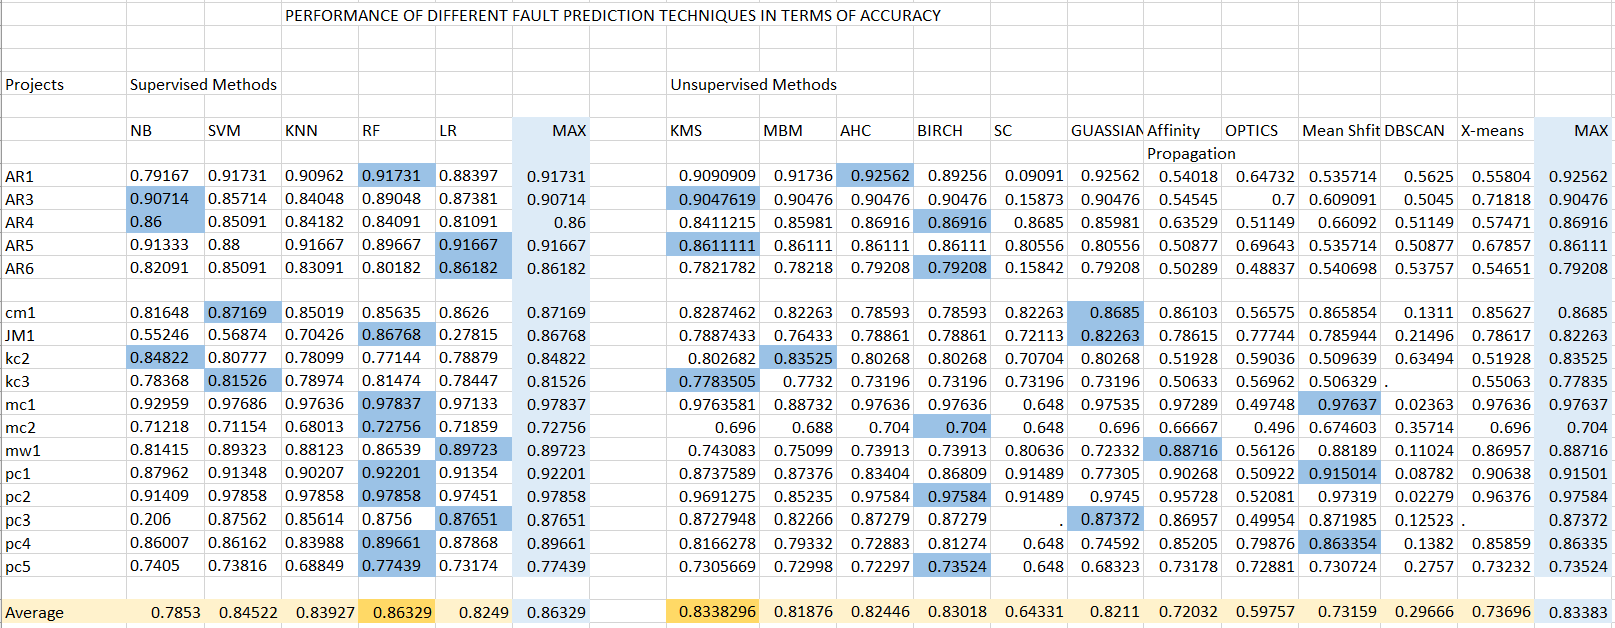
\includegraphics[scale=.6,keepaspectratio=true]{./accuracy}
\end{center}
\begin{table}[]
    \centering
    \caption{Performance of different algorithms in terms of accuracy}
    \label{tab:my_label}
\end{table}

\begin{center}
 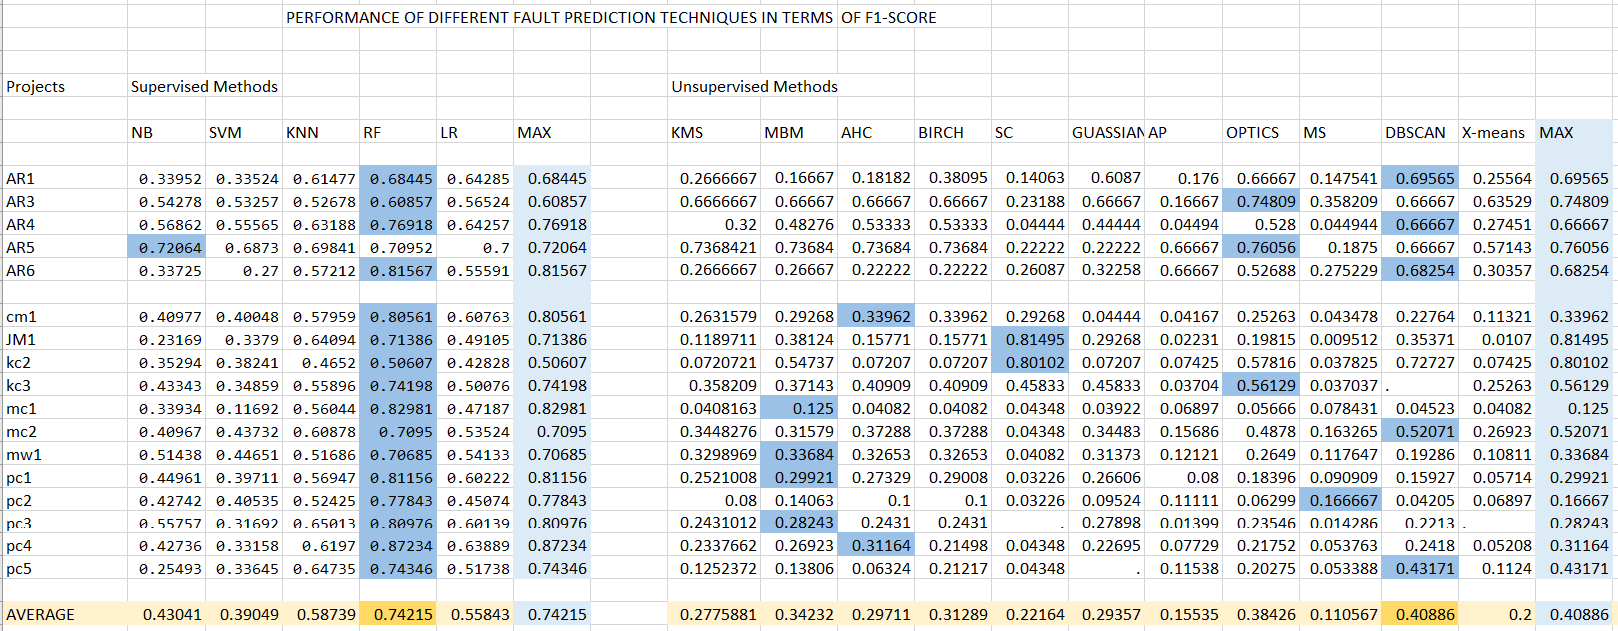
\includegraphics[scale=.5,keepaspectratio=true]{./f1score}
\end{center}
\begin{table}[]
    \centering
    \caption{Performance of different algorithms in terms of f1-score}
    \label{tab:my_label}
\end{table}

\begin{center}
 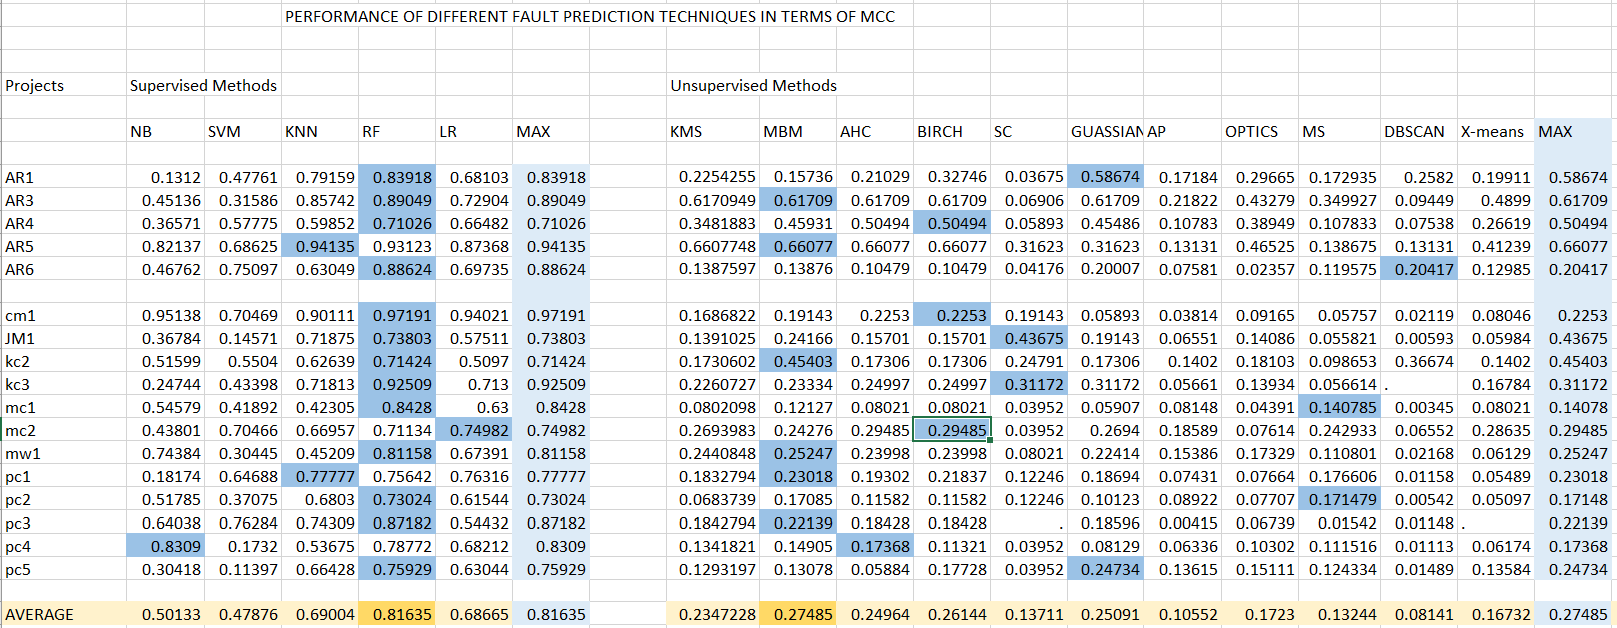
\includegraphics[scale=.5,keepaspectratio=true]{./mcc}
\end{center}
\begin{table}[]
    \centering
    \caption{Performance of different algorithms in terms of MCC}
\end{table}

\pagebreak

\noindent Fig 1 to Fig 17 depict the boxplots of 2 indicators of all supervised models for all 17 datasets.\newline

\begin{figure}[h!]
  \centering
  \begin{subfigure}[b]{0.4\linewidth}
    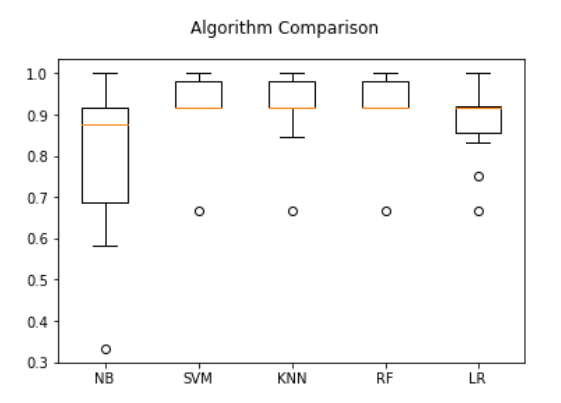
\includegraphics[width=\linewidth]{report/ar1.png}
    \caption{accuracy}
  \end{subfigure}
  \begin{subfigure}[b]{0.4\linewidth}
    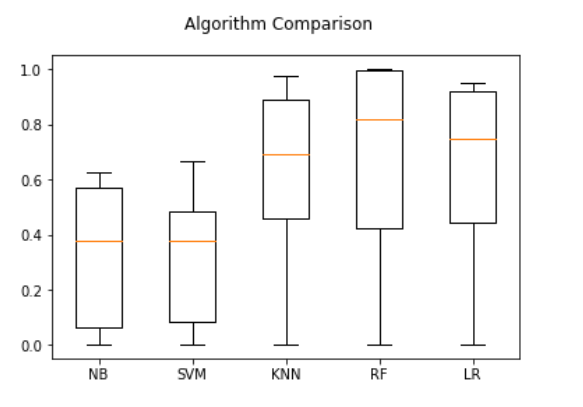
\includegraphics[width=\linewidth]{report/ar1_f.png}
    \caption{f1-score}
  \end{subfigure}
  \caption{Boxplots of supervised models on ar1 dataset}
\end{figure}

\begin{figure}[h!]
  \centering
  \begin{subfigure}[b]{0.4\linewidth}
    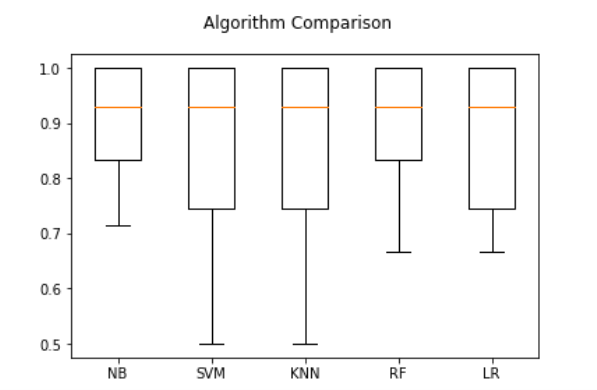
\includegraphics[width=\linewidth]{report/ar3.png}
    \caption{accuracy}
  \end{subfigure}
  \begin{subfigure}[b]{0.4\linewidth}
    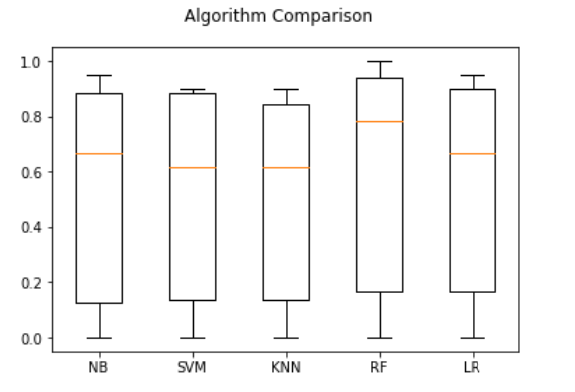
\includegraphics[width=\linewidth]{report/ar3_f.png}
    \caption{f1-score}
  \end{subfigure}
  \caption{Boxplots of supervised models on ar3 dataset}
\end{figure}

\begin{figure}[h!]
  \centering
  \begin{subfigure}[b]{0.4\linewidth}
    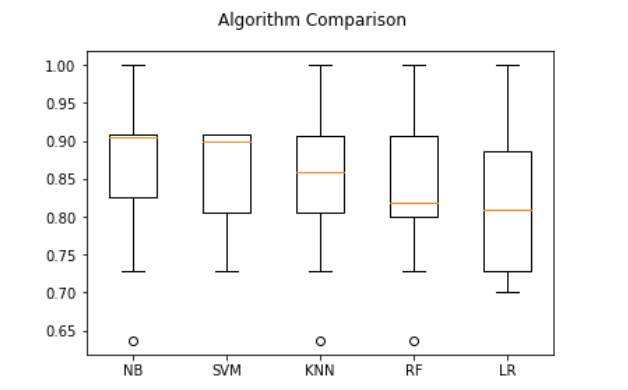
\includegraphics[width=\linewidth]{report/ar4.png}
    \caption{accuracy}
  \end{subfigure}
  \begin{subfigure}[b]{0.4\linewidth}
    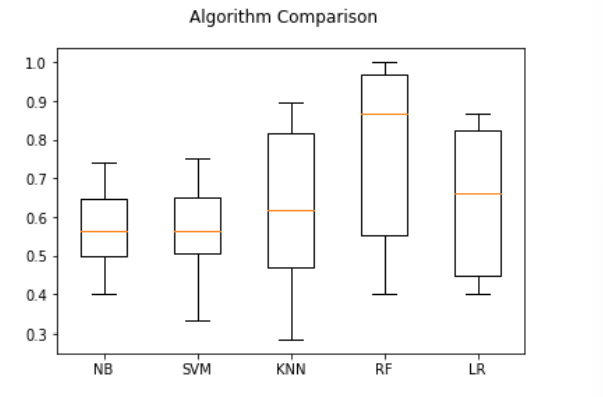
\includegraphics[width=\linewidth]{report/ar4_f.png}
    \caption{f1-score}
  \end{subfigure}
  \caption{Boxplots of supervised models on ar4 dataset}
\end{figure}

\pagebreak

\begin{figure}[h!]
  \centering
  \begin{subfigure}[b]{0.4\linewidth}
    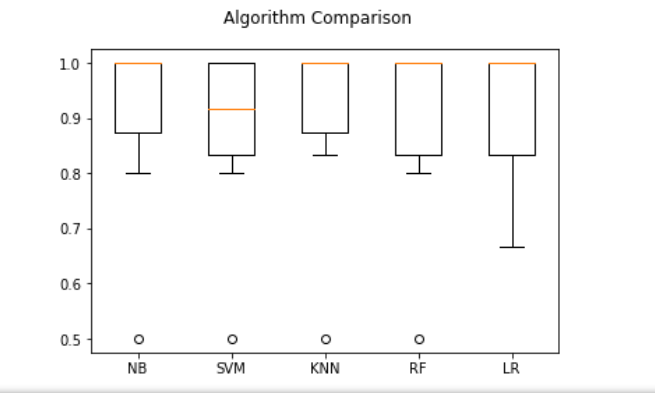
\includegraphics[width=\linewidth]{report/ar5.png}
    \caption{accuracy}
  \end{subfigure}
  \begin{subfigure}[b]{0.4\linewidth}
    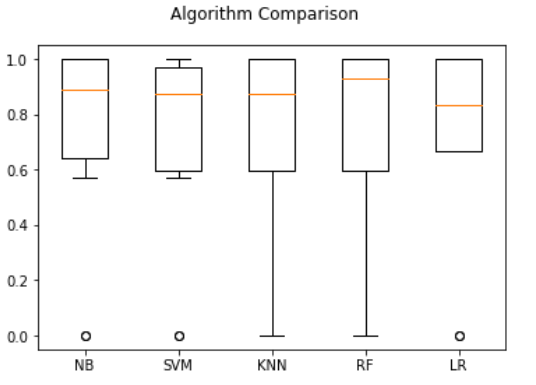
\includegraphics[width=\linewidth]{report/ar5_f.png}
    \caption{f1-score}
  \end{subfigure}
  \caption{Boxplots of supervised models on ar5 dataset}
\end{figure}

\begin{figure}[h!]
  \centering
  \begin{subfigure}[b]{0.4\linewidth}
    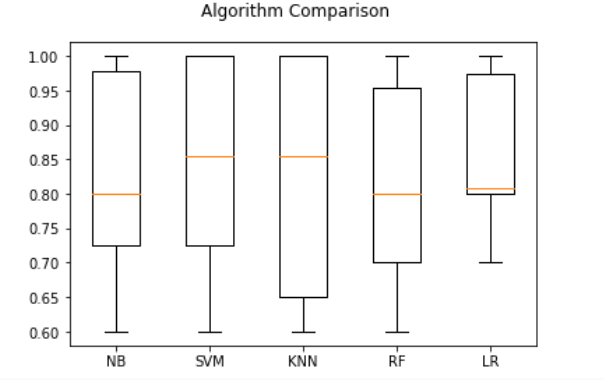
\includegraphics[width=\linewidth]{report/ar6.png}
    \caption{accuracy}
  \end{subfigure}
  \begin{subfigure}[b]{0.4\linewidth}
    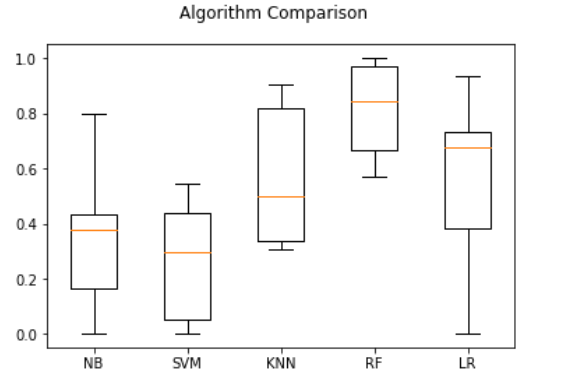
\includegraphics[width=\linewidth]{report/ar6_f.png}
    \caption{f1-score}
  \end{subfigure}
  \caption{Boxplots of supervised models on ar6 dataset}
\end{figure}

\begin{figure}[h!]
  \centering
  \begin{subfigure}[b]{0.4\linewidth}
    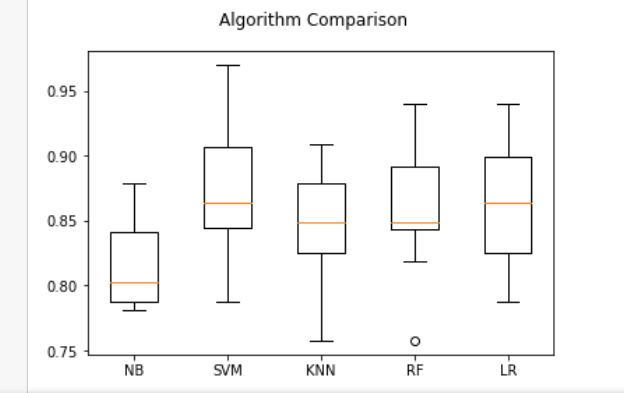
\includegraphics[width=\linewidth]{report/cm1.png}
    \caption{accuracy}
  \end{subfigure}
  \begin{subfigure}[b]{0.4\linewidth}
    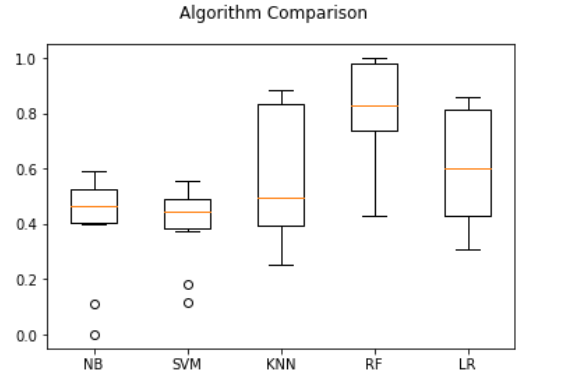
\includegraphics[width=\linewidth]{report/cm1_f.png}
    \caption{f1-score}
  \end{subfigure}
  \caption{Boxplots of supervised models on cm1 dataset}
\end{figure}

\pagebreak

\begin{figure}[h!]
  \centering
  \begin{subfigure}[b]{0.4\linewidth}
    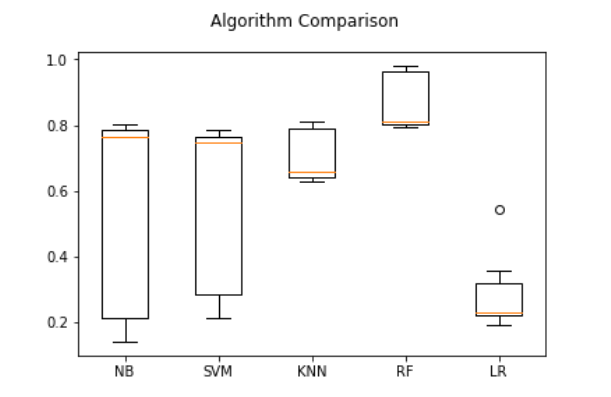
\includegraphics[width=\linewidth]{report/JM1.png}
    \caption{accuracy}
  \end{subfigure}
  \begin{subfigure}[b]{0.4\linewidth}
    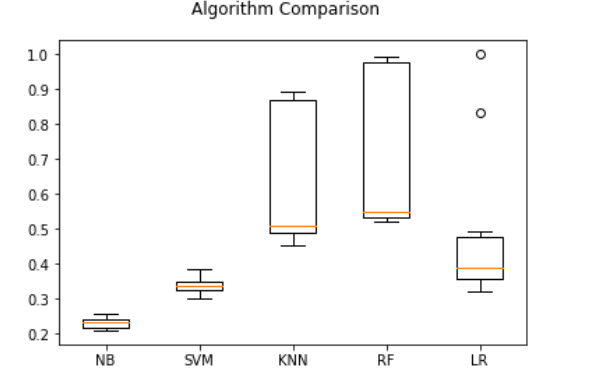
\includegraphics[width=\linewidth]{report/JM1_f.png}
    \caption{f1-score}
  \end{subfigure}
  \caption{Boxplots of supervised models on JM1 dataset}
\end{figure}

\begin{figure}[h!]
  \centering
  \begin{subfigure}[b]{0.4\linewidth}
    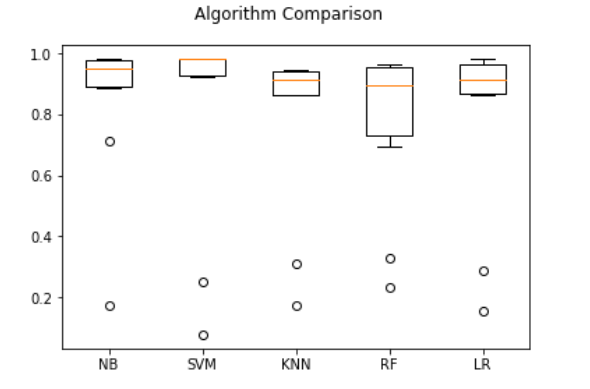
\includegraphics[width=\linewidth]{report/kc2.png}
    \caption{accuracy}
  \end{subfigure}
  \begin{subfigure}[b]{0.4\linewidth}
    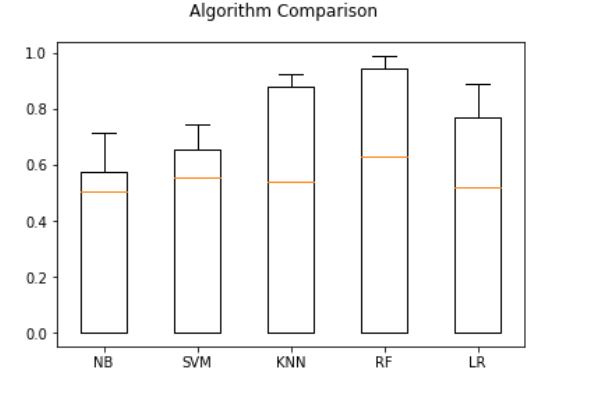
\includegraphics[width=\linewidth]{report/kc2_f.png}
    \caption{f1-score}
  \end{subfigure}
  \caption{Boxplots of supervised models on kc2 dataset}
\end{figure}

\begin{figure}[h!]
  \centering
  \begin{subfigure}[b]{0.4\linewidth}
    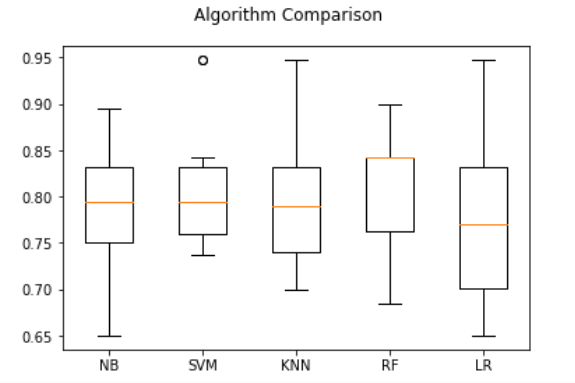
\includegraphics[width=\linewidth]{report/KC3.png}
    \caption{accuracy}
  \end{subfigure}
  \begin{subfigure}[b]{0.4\linewidth}
    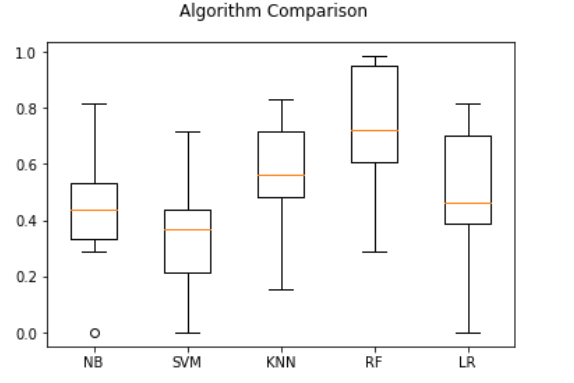
\includegraphics[width=\linewidth]{report/KC3_f.png}
    \caption{f1-score}
  \end{subfigure}
  \caption{Boxplots of supervised models on KC3 dataset}
\end{figure}

\pagebreak

\begin{figure}[h!]
  \centering
  \begin{subfigure}[b]{0.4\linewidth}
    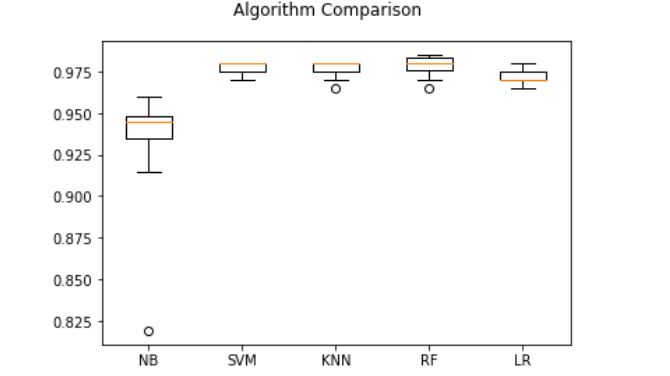
\includegraphics[width=\linewidth]{report/mc1.png}
    \caption{accuracy}
  \end{subfigure}
  \begin{subfigure}[b]{0.4\linewidth}
    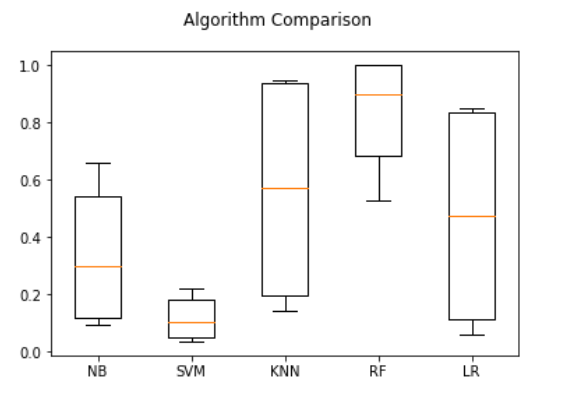
\includegraphics[width=\linewidth]{report/mc1_f.png}
    \caption{f1-score}
  \end{subfigure}
  \caption{Boxplots of supervised models on mc1 dataset}
\end{figure}

\begin{figure}[h!]
  \centering
  \begin{subfigure}[b]{0.4\linewidth}
    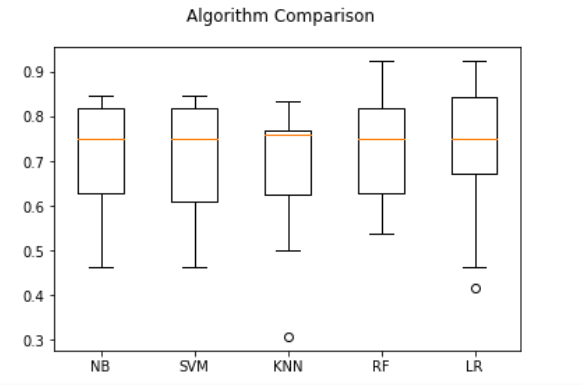
\includegraphics[width=\linewidth]{report/mc2.png}
    \caption{accuracy}
  \end{subfigure}
  \begin{subfigure}[b]{0.4\linewidth}
    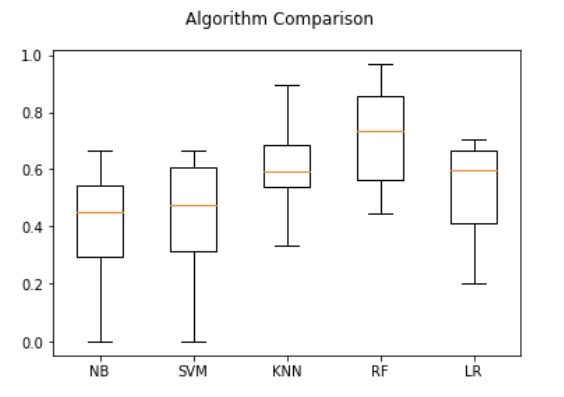
\includegraphics[width=\linewidth]{report/mc2_f.png}
    \caption{f1-score}
  \end{subfigure}
  \caption{Boxplots of supervised models on mc2 dataset}
\end{figure}

\begin{figure}[h!]
  \centering
  \begin{subfigure}[b]{0.4\linewidth}
    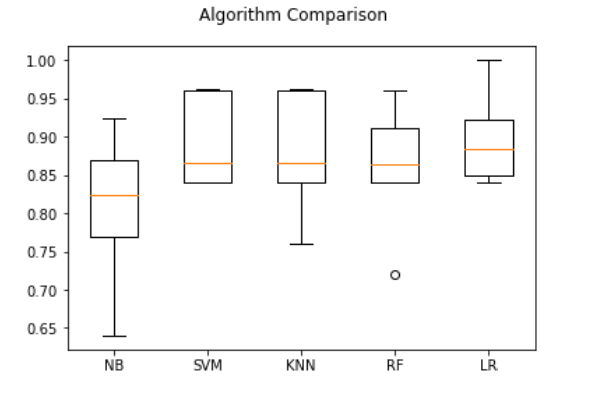
\includegraphics[width=\linewidth]{report/mw1.png}
    \caption{accuracy}
  \end{subfigure}
  \begin{subfigure}[b]{0.4\linewidth}
    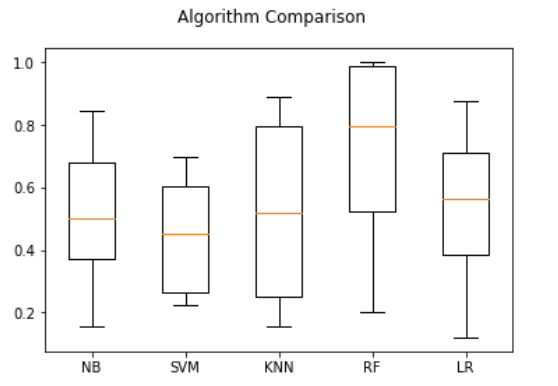
\includegraphics[width=\linewidth]{report/mw1_f.png}
    \caption{f1-score}
  \end{subfigure}
  \caption{Boxplots of supervised models on mw1 dataset}
\end{figure}

\pagebreak

\begin{figure}[h!]
  \centering
  \begin{subfigure}[b]{0.4\linewidth}
    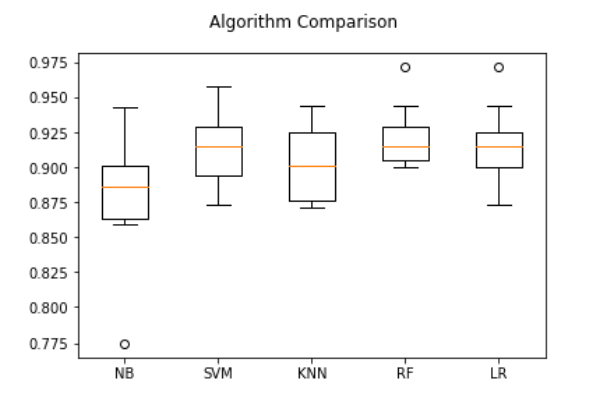
\includegraphics[width=\linewidth]{report/PC1.png}
    \caption{accuracy}
  \end{subfigure}
  \begin{subfigure}[b]{0.4\linewidth}
    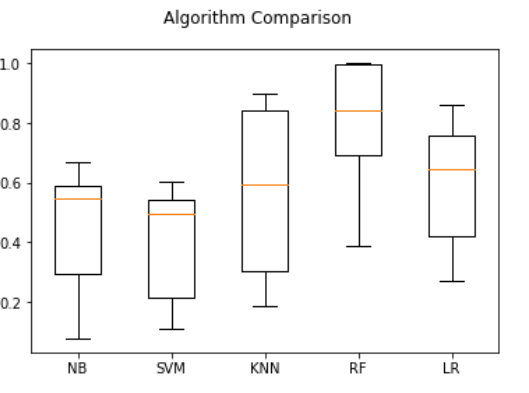
\includegraphics[width=\linewidth]{report/PC1_f.png}
    \caption{f1-score}
  \end{subfigure}
  \caption{Boxplots of supervised models on PC1 dataset}
\end{figure}

\begin{figure}[h!]
  \centering
  \begin{subfigure}[b]{0.4\linewidth}
    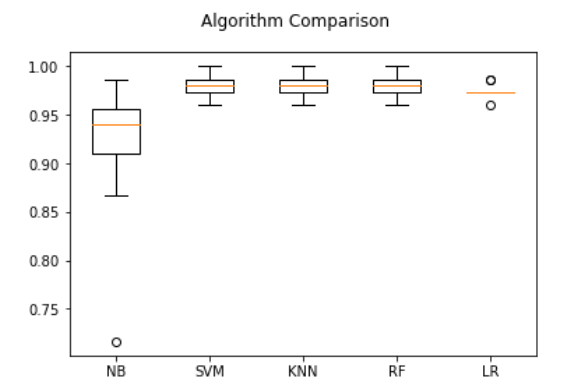
\includegraphics[width=\linewidth]{report/PC2.png}
    \caption{accuracy}
  \end{subfigure}
  \begin{subfigure}[b]{0.4\linewidth}
    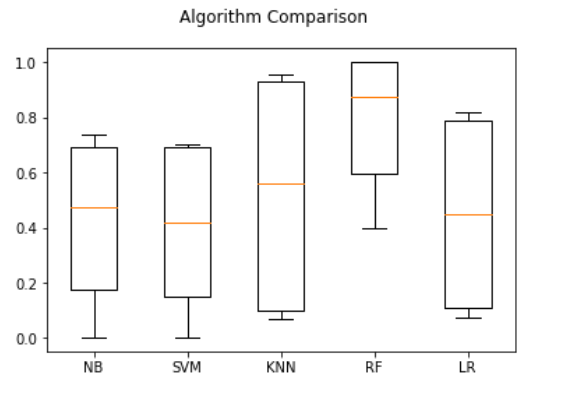
\includegraphics[width=\linewidth]{report/PC2_f.png}
    \caption{f1-score}
  \end{subfigure}
  \caption{Boxplots of supervised models on PC2 dataset}
\end{figure}

\begin{figure}[h!]
  \centering
  \begin{subfigure}[b]{0.4\linewidth}
    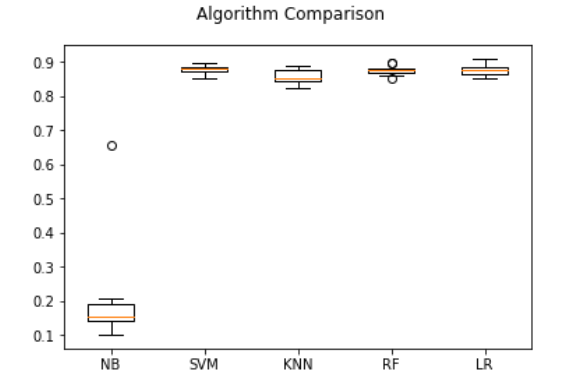
\includegraphics[width=\linewidth]{report/PC3.png}
    \caption{accuracy}
  \end{subfigure}
  \begin{subfigure}[b]{0.4\linewidth}
    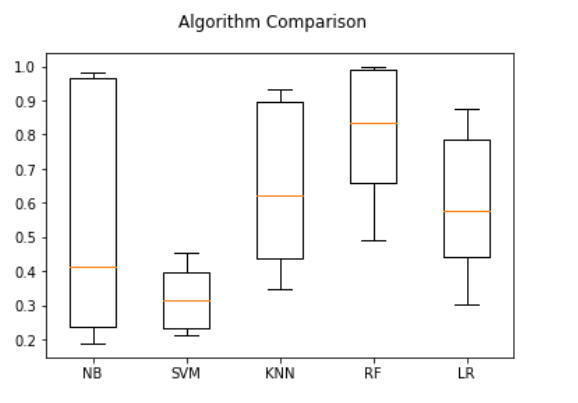
\includegraphics[width=\linewidth]{report/PC3_f.png}
    \caption{f1-score}
  \end{subfigure}
  \caption{Boxplots of supervised models on PC3 dataset}
\end{figure}

\pagebreak

\begin{figure}[h!]
  \centering
  \begin{subfigure}[b]{0.4\linewidth}
    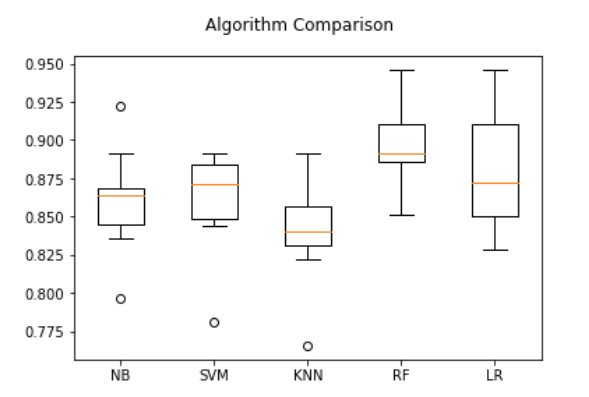
\includegraphics[width=\linewidth]{report/PC4.png}
    \caption{accuracy}
  \end{subfigure}
  \begin{subfigure}[b]{0.4\linewidth}
    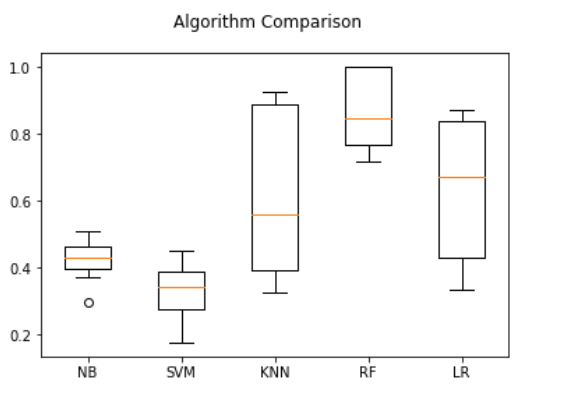
\includegraphics[width=\linewidth]{report/PC4_f.png}
    \caption{f1-score}
  \end{subfigure}
  \caption{Boxplots of supervised models on PC4 dataset}
\end{figure}

\begin{figure}[h!]
  \centering
  \begin{subfigure}[b]{0.4\linewidth}
    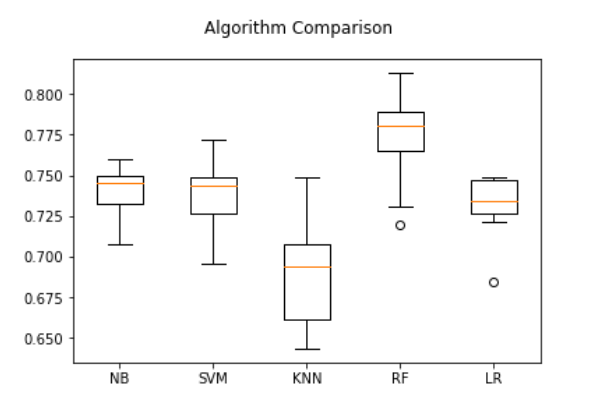
\includegraphics[width=\linewidth]{report/PC5.png}
    \caption{accuracy}
  \end{subfigure}
  \begin{subfigure}[b]{0.4\linewidth}
    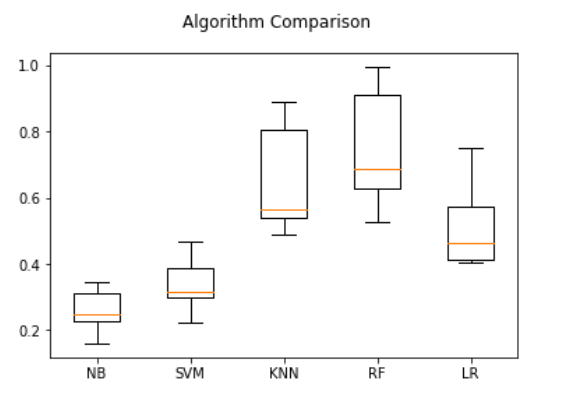
\includegraphics[width=\linewidth]{report/PC5_f.png}
    \caption{f1-score}
  \end{subfigure}
  \caption{Boxplots of supervised models on PC5 dataset}
\end{figure}

\pagebreak

\noindent 1. \underline{In terms of accuracy}\newline
From Table 3.1, we can observe that, for a particular dataset -
In supervised model family except KNN all other models performed well.Also Random Forest (RF) performed best among all other models.In unsupervised models, KMS, BIRCH, Guassian and MS models performed better than other models.\newline
If we talk about average performance of each model over all datasets, Rf is the best model among all supervised clustering models and KMS performed best among all unsupervised models.\newline

\noindent 2. \underline{In terms of f1-score}\newline
From Table 3.2, for a particular dataset, we can say that among all classifiers in the supervised model family RF outperformed other models. Also we can place KNN at second position. In unsupervised model family, MBM, OPTICS and DBSCAN performed better than other models.\newline
If we see average performance of these models, RF is the best model in supervised model family and DBSCAN performed better in unsupervised model family.\newline

\noindent 2. \underline{In terms of MCC}\newline
From Table 3.3, we observe that, for a particular dataset among all classifiers in the supervised model family RF performed best. In unsupervised model family, MBM, BIRCH and Guassian performed better than other models.\newline
If we see average performance of these models, RF is the best model in supervised model family and MBM performed better in unsupervised model family.






\chapter{Conclusions and Discussion}\label{final}

We conducted a small-scale comparison to analyze SDP performance differences among 11 clustering-based unsupervised models and 5 typical supervised models. We made the first step towards investigating the impacts of the feature types of defect data on the performance of these methods. Since the defect data was highly imbalanced so we also used oversampling methods to balance the data.\newline
Our experimental results on 17 defect data indicate that not all clustering-based unsupervised models are worse than the supervised models.\newline
Firstly we are using accuracy performance indicator-\newline
If we compare supervised algorithms only, RF performed better over other algorithms. In unsupervised models , KMS model performed better over other models.\newline
If we see MCC performance of our models we find that RF in supervised model family and MBM in unsupervised model family performed better.\newline
But when we have an imbalanced data ,accuracy is not a good metric.
So we are making conclusion on the basis of f1-score.\newline
To sum up, on defect data we can say that Random Forest in supervised model family and DBSCAN in  unsupervised model family performed best on f1-score performance indicator.


\bibliographystyle{IEEEtran}
\bibliography{report}
\end{document}
